\chapter{Évaluation, validation et analyse}
\label{chap:eval_valid_modele}

\lipsum[1]

\localtableofcontents

\newpage

% -----------------------------------------------------------------------------
\section{Évaluation sur le dataset de test}
\section{Évaluation sur le dataset de test}

\subsection{Protocole d'évaluation}

L'évaluation des modèles a été réalisée sur un dataset de test indépendant composé de 89 images représentatives du canton de Genève. Cette évaluation porte sur 93 configurations distinctes, comprenant 89 modèles issus de Segmentation Models PyTorch (SMP) et 4 variantes de YOLOv12. Pour garantir la robustesse des résultats, chaque configuration a été entraînée selon une validation croisée à 5 plis, permettant d'obtenir des performances moyennées et des écarts-types significatifs.

\subsubsection{Métriques d'évaluation}

Les performances des modèles ont été évaluées selon plusieurs métriques complémentaires :

\begin{itemize}
    \item \textbf{IoU (Intersection over Union)} : métrique principale mesurant le recouvrement entre les prédictions et les annotations de référence
    \item \textbf{mAP@k} : précision moyenne à différents seuils d'IoU (50\%, 55\%, ..., 95\%)
    \item \textbf{F1-score} : moyenne harmonique entre précision et rappel
    \item \textbf{Métriques classiques} : précision, rappel et exactitude
\end{itemize}

Les aspects computationnels ont également été mesurés :
\begin{itemize}
    \item Temps d'entraînement total pour les 5 plis
    \item Nombre de paramètres du modèle (en millions)
\end{itemize}

\subsection{Vue d'ensemble des performances}

\subsubsection{Distribution globale des résultats}

Les 93 modèles évalués présentent des performances IoU s'échelonnant de 0,583 à 0,742, avec une moyenne de 0,708 et un écart-type de 0,024. Cette faible dispersion témoigne de la qualité générale des architectures modernes de segmentation sur cette tâche spécifique.

La Figure~\ref{fig:heatmap_iou} présente une vue synthétique des performances pour chaque combinaison encodeur-décodeur. Les meilleures performances sont concentrées autour de certaines combinaisons privilégiées, notamment :

\begin{itemize}
    \item UNet++ avec les encodeurs EfficientNet (IoU > 0,73)
    \item DeepLabV3+ avec EfficientNetV2 (IoU > 0,72)
    \item UPerNet avec certains encodeurs RegNetY
\end{itemize}

\begin{figure}[htbp]
    \centering
    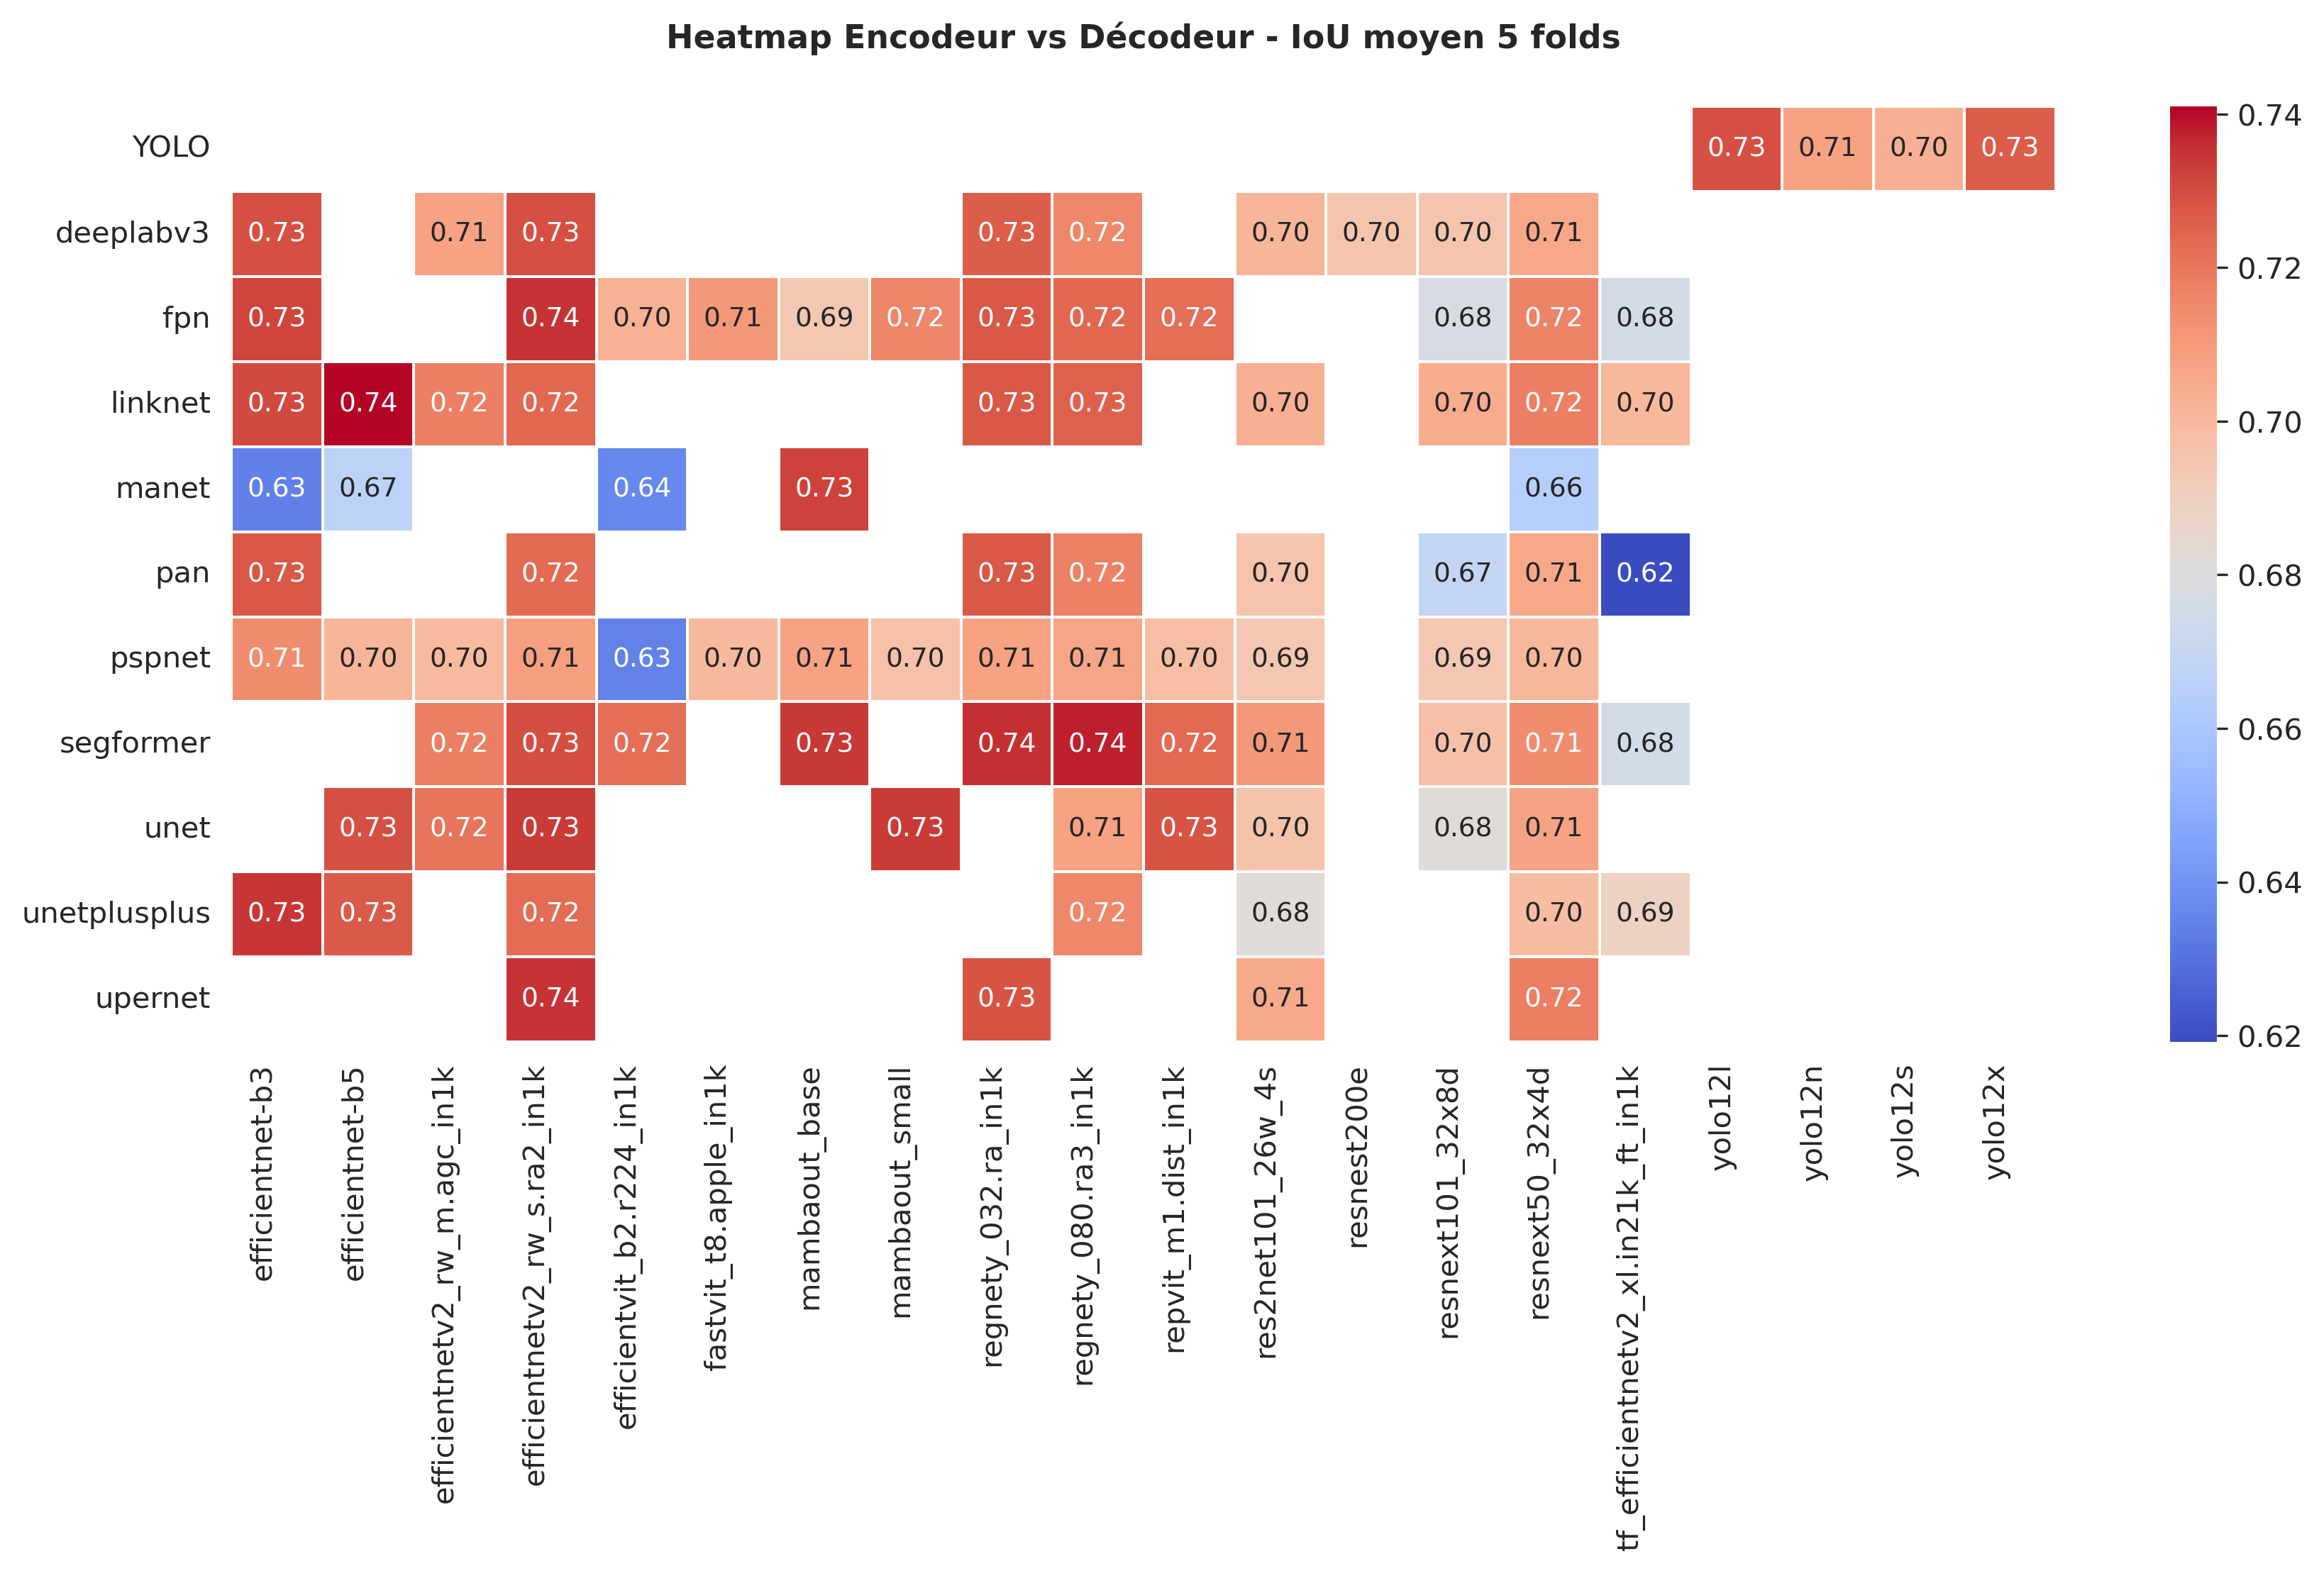
\includegraphics[width=\textwidth]{ch4_01_architecture_backbone_heatmap_01_eval_test_iou_mean.png}
    \caption{Matrice de performance IoU par combinaison encodeur-décodeur. Les cases vides indiquent des combinaisons non testées ou ayant échoué durant l'entraînement.}
    \label{fig:heatmap_iou}
\end{figure}

\subsubsection{Top 10 des modèles}

Le Tableau~\ref{tab:top5_modeles} présente les 5 meilleurs modèles selon l'IoU moyen sur les 5 plis :

\begin{table}[htbp]
    \centering
    \caption{Top 5 des modèles par IoU moyen sur dataset de test}
    \begin{tabular}{lccccc}
        \toprule
        Modèle & IoU & F1-Score & Params (M) & Temps (h) \\
        \midrule
        UNet++ + tu-fastvit\_t8 & 0,742 & 0,814 & 15,2 & 14,8 \\
        DeepLabV3+ + EfficientNetV2-S & 0,729 & 0,800 & 22,5 & 18,5 \\
        DeepLabV3+ + EfficientNet-B3 & 0,729 & 0,797 & 11,7 & 30,9 \\
        YOLO12l & 0,729 & 0,587 & 28,8 & 23,1 \\
        DeepLabV3+ + RegNetY-032 & 0,727 & 0,795 & 20,4 & 30,4 \\
        \bottomrule
    \end{tabular}
    \label{tab:top5_modeles}
\end{table}

Plusieurs observations émergent de cette analyse :
\begin{itemize}
    \item Les architectures UNet++ et DeepLabV3+ dominent le classement
    \item Les modèles YOLO, bien que compétitifs en IoU, présentent des F1-scores significativement inférieurs
    \item Les temps d'entraînement varient considérablement (14,8h à 30,9h) sans corrélation directe avec les performances
\end{itemize}

\subsection{Analyse comparative des architectures}

\subsubsection{Performance par famille de décodeur}

L'analyse des performances par architecture (Figure~\ref{fig:boxplot_arch}) révèle des différences notables entre les familles de décodeurs :

\begin{figure}[htbp]
    \centering
    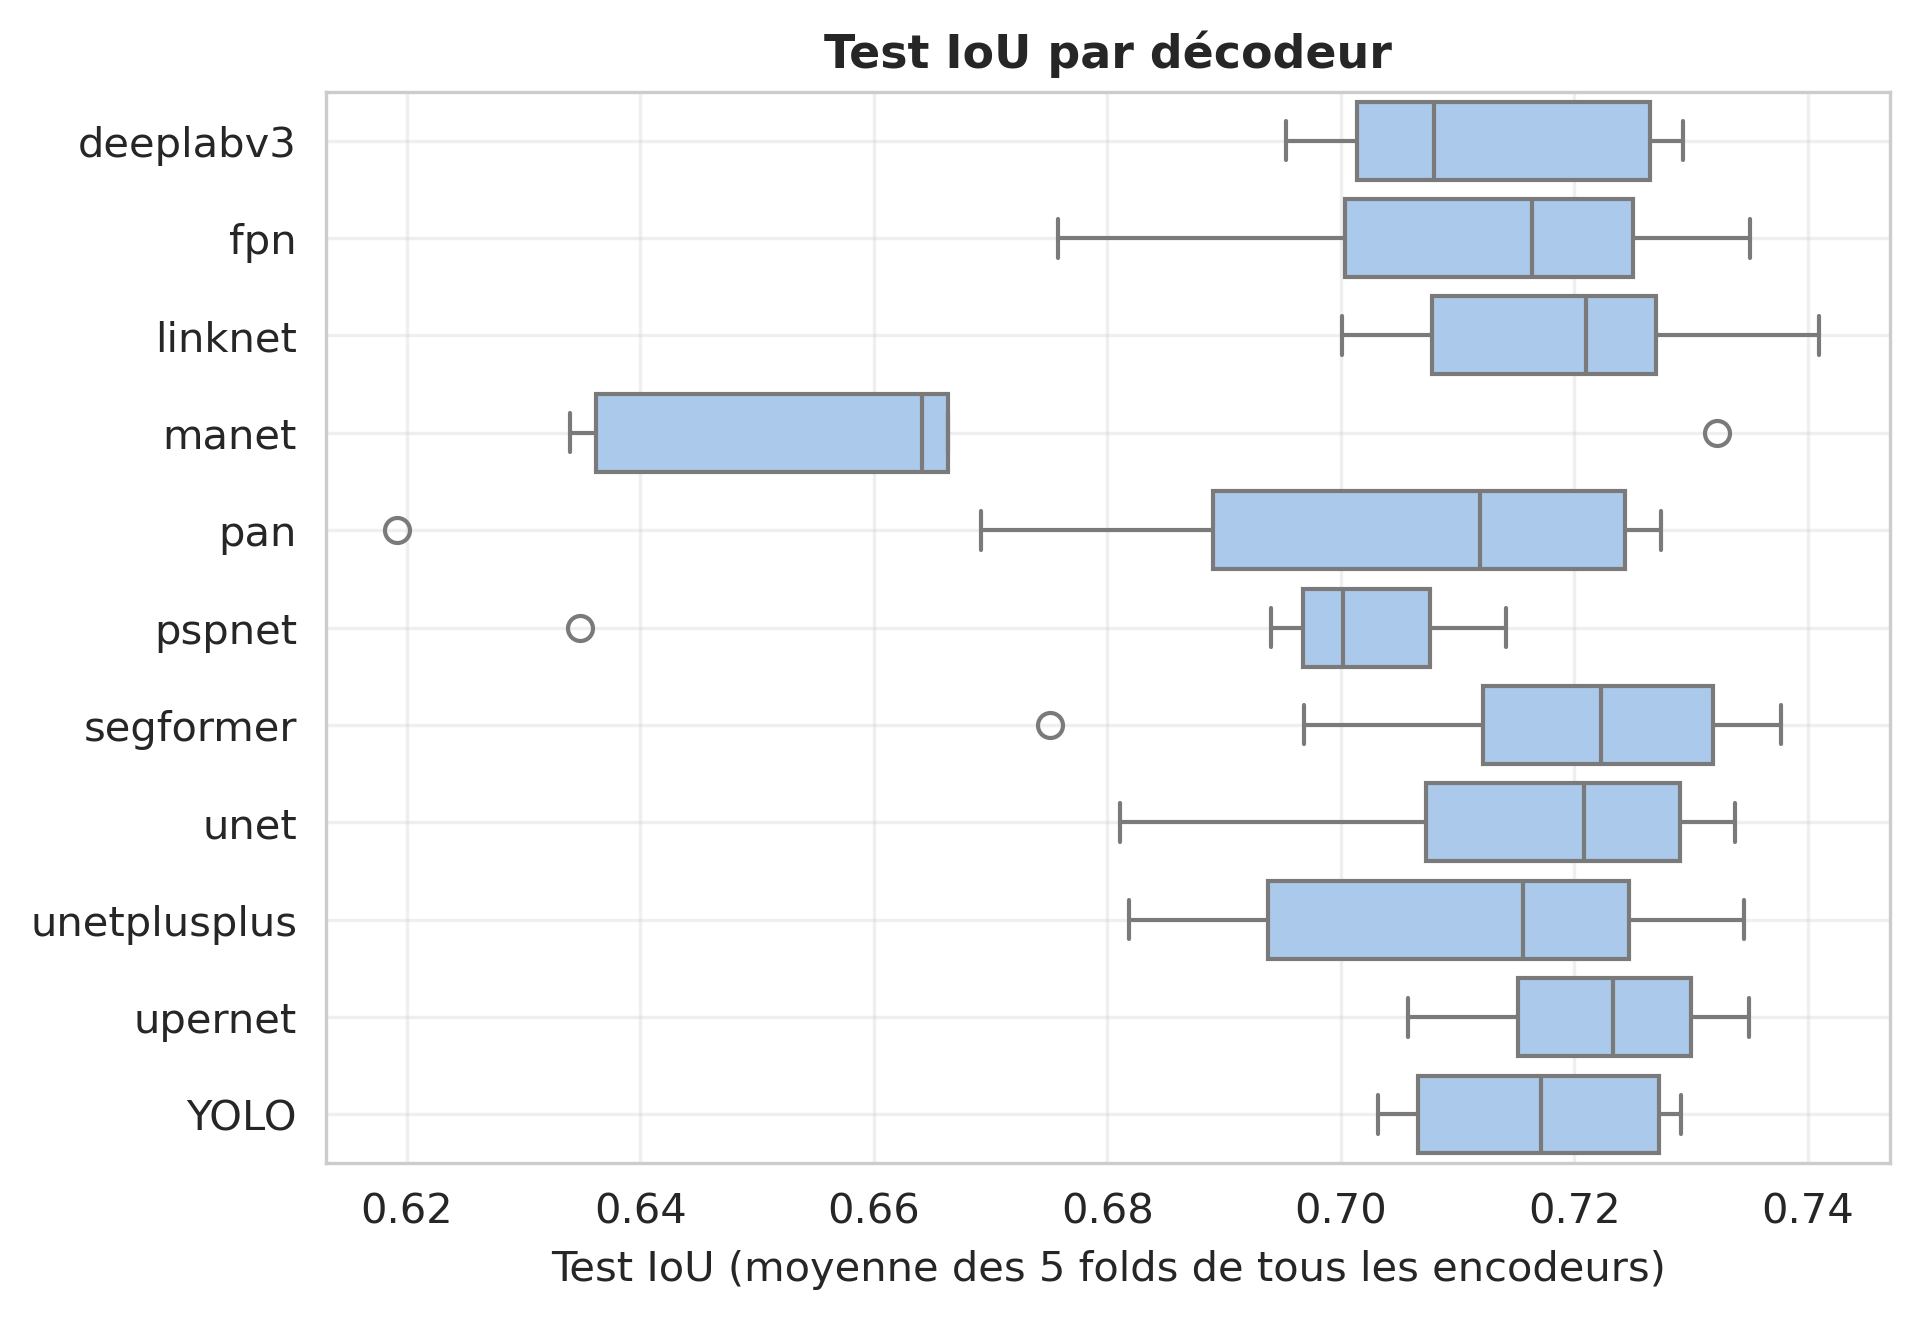
\includegraphics[width=0.8\textwidth]{ch4_06_architecture_boxplot_01_eval_test_iou_mean.png}
    \caption{Distribution des performances IoU par architecture de décodeur}
    \label{fig:boxplot_arch}
\end{figure}

Les architectures peuvent être classées en trois catégories selon leurs performances :

\textbf{Haute performance (IoU > 0,71)} :
\begin{itemize}
    \item \textbf{UNet++} : Médiane la plus élevée (0,724) avec la plus faible variance, démontrant une robustesse remarquable
    \item \textbf{YOLO} : Performances compétitives mais variance plus importante
    \item \textbf{DeepLabV3+} : Excellentes performances moyennes avec quelques outliers
\end{itemize}

\textbf{Performance intermédiaire (0,69 < IoU < 0,71)} :
\begin{itemize}
    \item \textbf{UPerNet, DPT, MANet} : Architectures complexes avec résultats variables selon l'encodeur
    \item \textbf{SegFormer} : Architecture Transformer moderne mais sans avantage décisif sur cette tâche
\end{itemize}

\textbf{Performance modérée (IoU < 0,69)} :
\begin{itemize}
    \item \textbf{FPN, LinkNet} : Architectures plus légères sacrifiant la précision pour la vitesse
    \item \textbf{PAN} : Performances décevantes malgré sa complexité théorique
\end{itemize}

\subsubsection{Performance par encodeur}

L'analyse des encodeurs (Figure~\ref{fig:top_encodeurs}) montre l'importance cruciale du choix de l'extracteur de caractéristiques :

\begin{figure}[htbp]
    \centering
    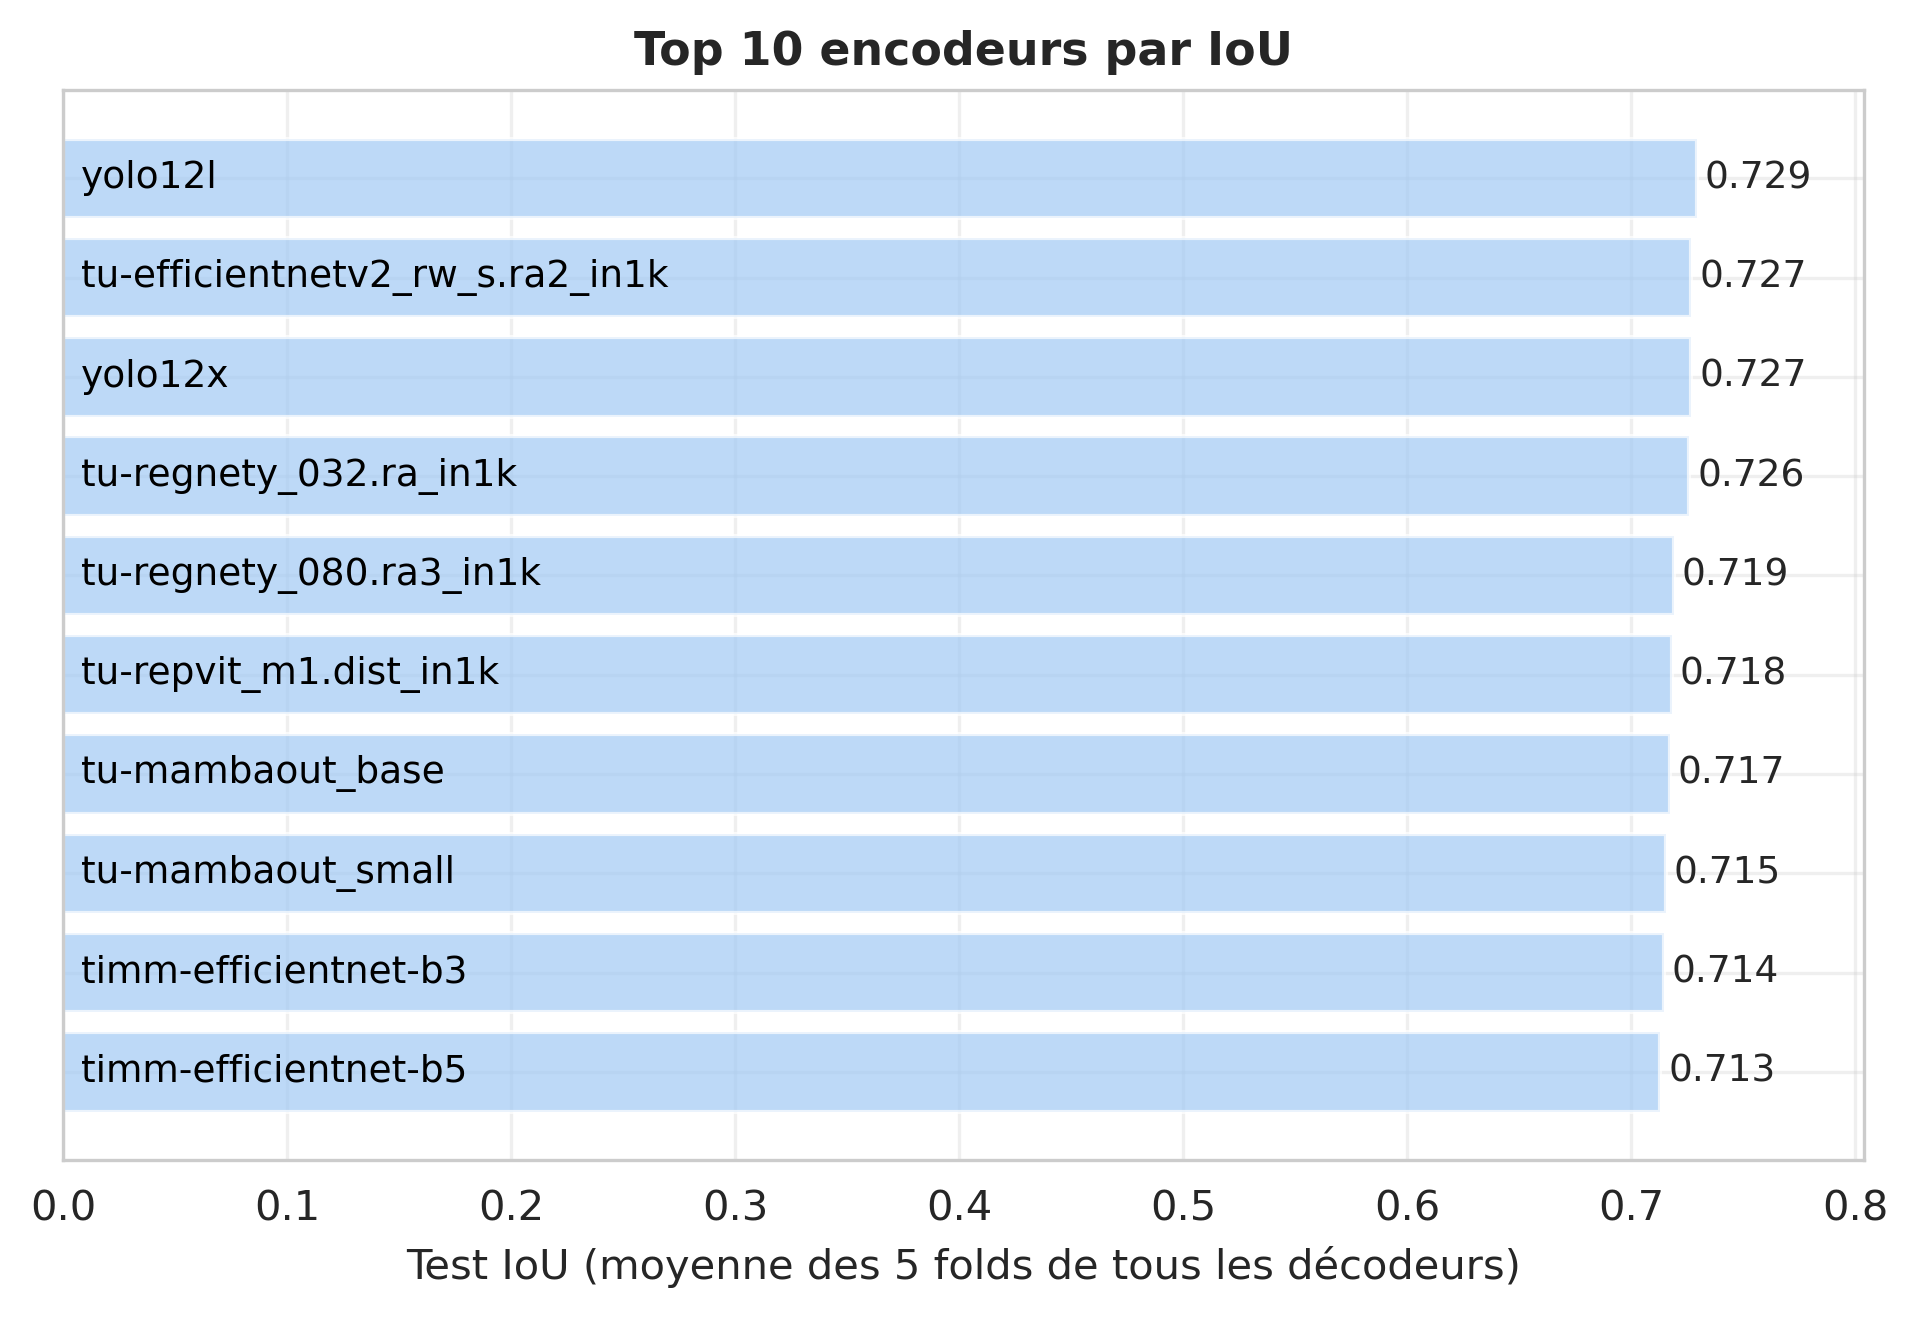
\includegraphics[width=0.8\textwidth]{ch4_04_backbone_performance_01_eval_test_iou_mean.png}
    \caption{Top 10 des encodeurs par IoU moyen (tous décodeurs confondus)}
    \label{fig:top_encodeurs}
\end{figure}

Les encodeurs les plus performants partagent plusieurs caractéristiques :
\begin{itemize}
    \item \textbf{Architectures récentes} : FastViT (2023), EfficientNetV2 (2021), RepViT (2024)
    \item \textbf{Optimisation mobile} : Plusieurs encodeurs conçus pour l'efficacité (FastViT, RepViT, MobileNetV3)
    \item \textbf{Pré-entraînement ImageNet} : Tous bénéficient du transfert d'apprentissage
\end{itemize}

\subsection{Analyse de l'efficacité computationnelle}

\subsubsection{Compromis performance-complexité}

L'analyse du front de Pareto (Figure~\ref{fig:pareto_params}) identifie les modèles offrant le meilleur compromis entre performance et complexité :

\begin{figure}[htbp]
    \centering
    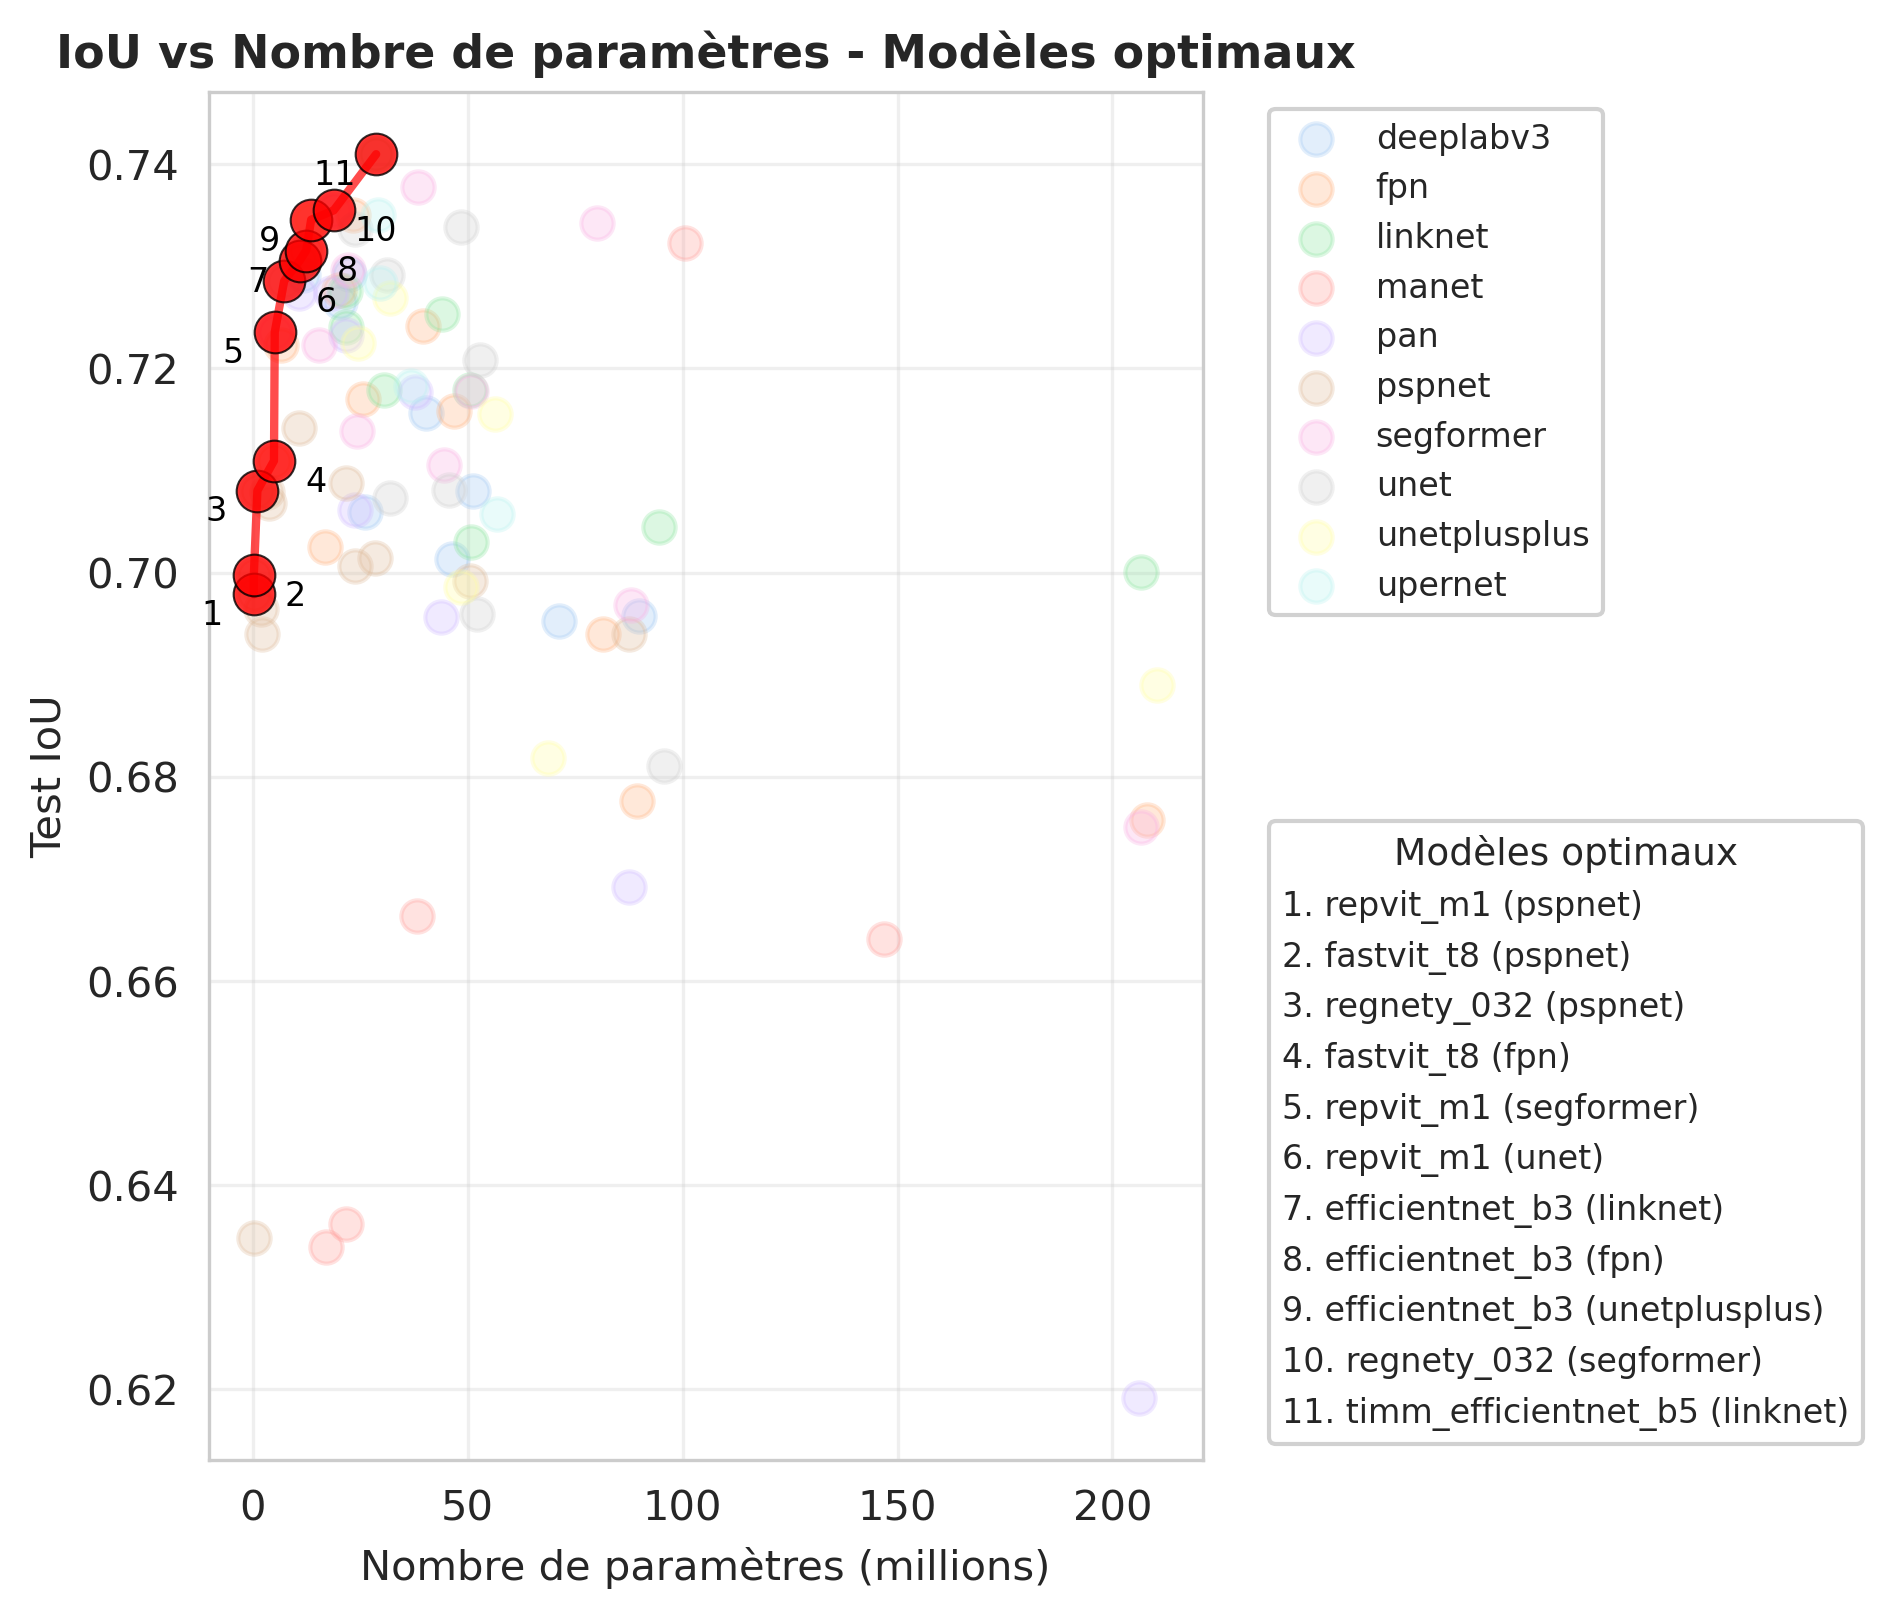
\includegraphics[width=\textwidth]{ch4_09_performance_vs_parameters_pareto_01_eval_test_iou_mean.png}
    \caption{Front de Pareto : IoU vs nombre de paramètres. Les modèles sur la ligne rouge représentent les solutions optimales.}
    \label{fig:pareto_params}
\end{figure}

Les modèles optimaux identifiés sont :
\begin{enumerate}
    \item \textbf{YOLO12n} (2,8M params) : Solution ultra-légère avec IoU acceptable (0,708)
    \item \textbf{UNet + MobileNetV3-large} (7,0M) : Excellent compromis taille/performance
    \item \textbf{DeepLabV3+ + EfficientNet-B3} (11,7M) : Performances élevées avec taille raisonnable
    \item \textbf{UNet++ + FastViT-T8} (15,2M) : Meilleures performances absolues
\end{enumerate}

Au-delà de 25M paramètres, les gains en performance deviennent marginaux (<1\% IoU), suggérant une saturation du bénéfice apporté par la complexité additionnelle.

\subsubsection{Analyse temporelle}

La distribution des temps d'entraînement (Figure~\ref{fig:training_time_dist}) révèle une forte hétérogénéité :

\begin{figure}[htbp]
    \centering
    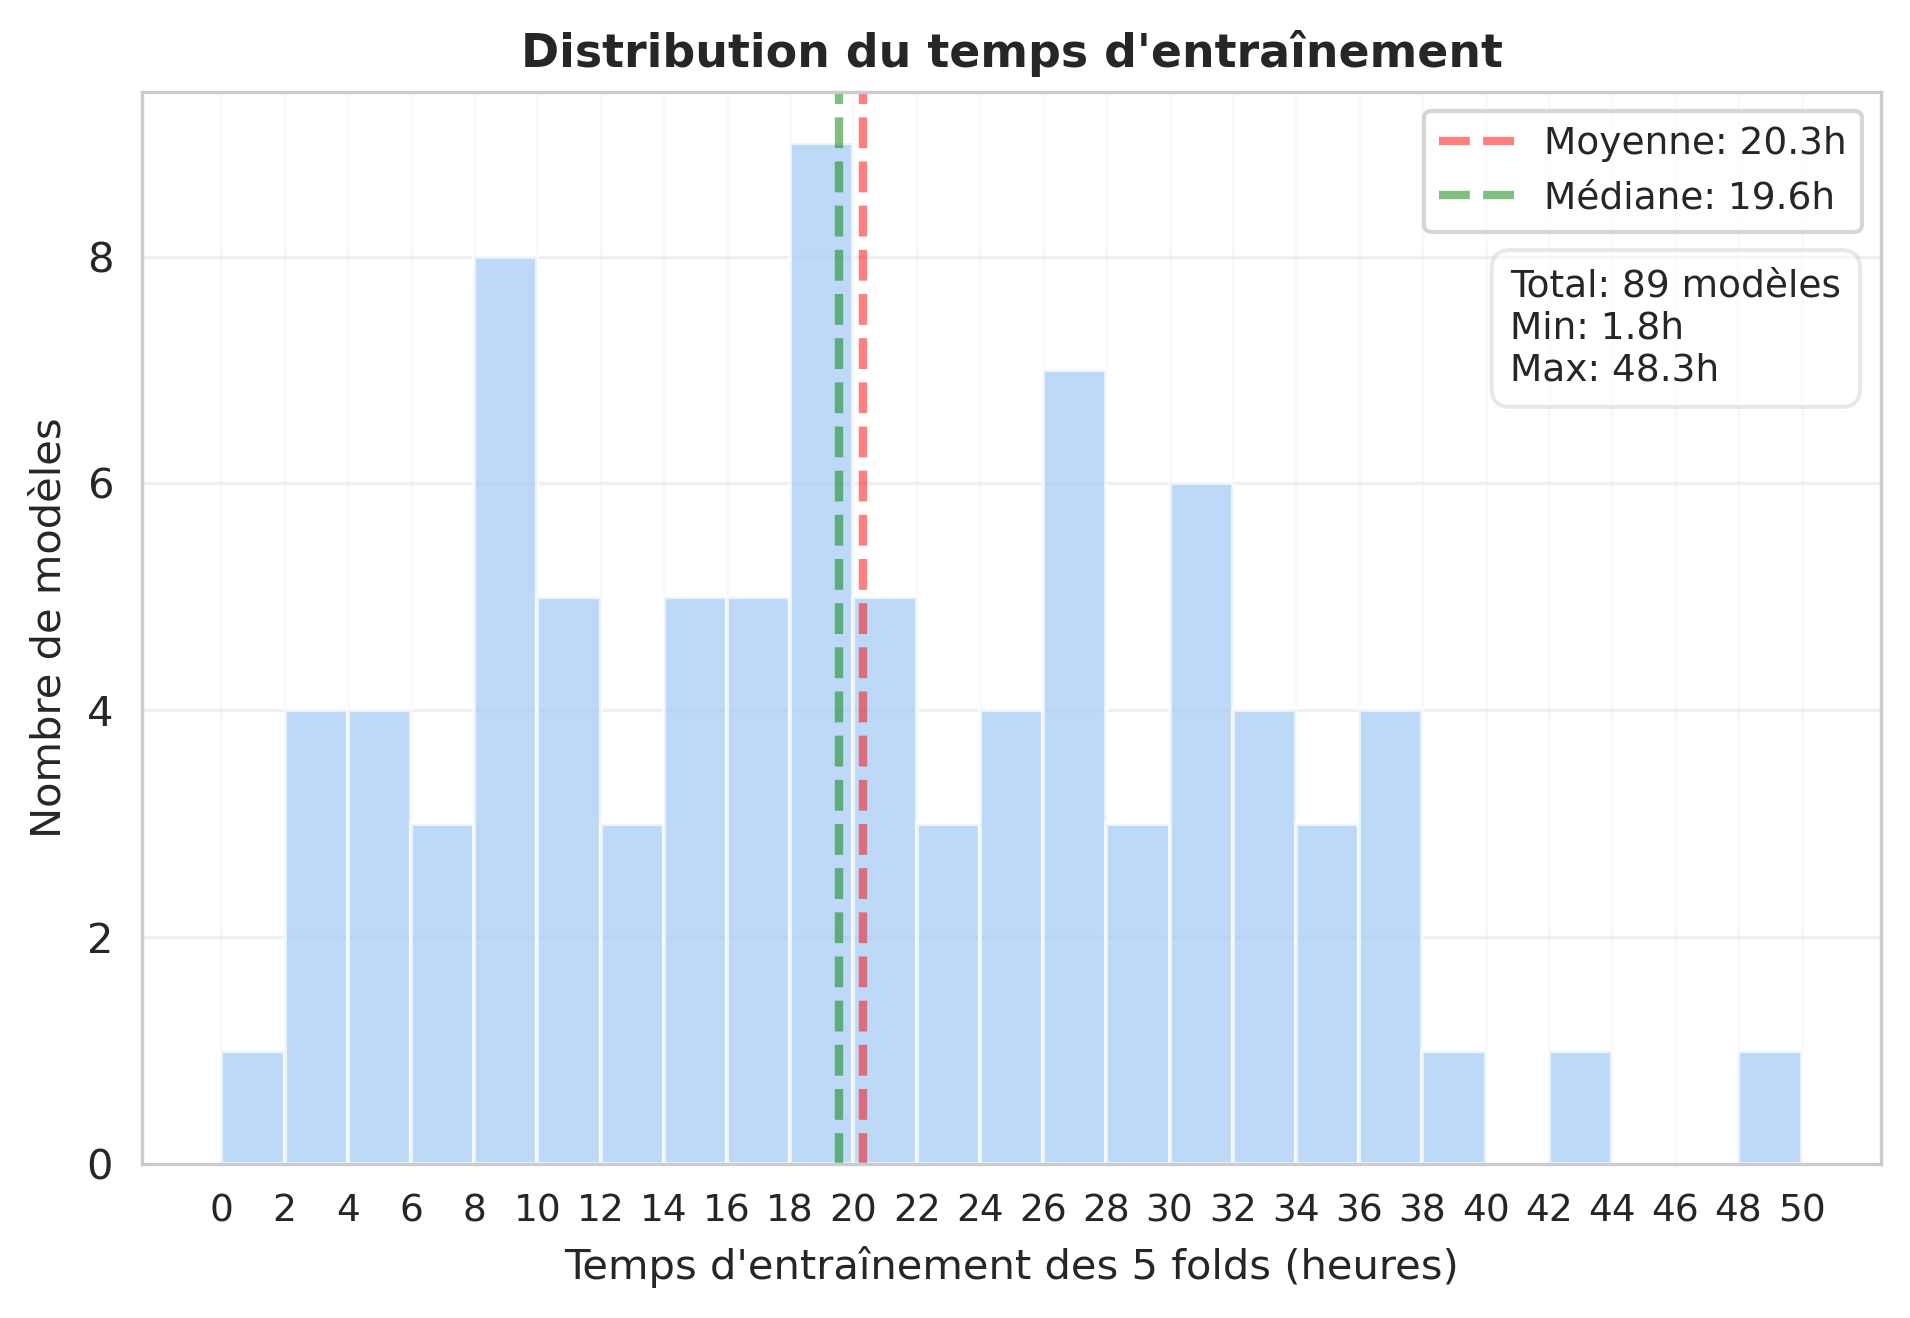
\includegraphics[width=0.8\textwidth]{ch4_11_training_time_dist_09.png}
    \caption{Distribution du temps d'entraînement total (5 plis)}
    \label{fig:training_time_dist}
\end{figure}

Les observations principales sont :
\begin{itemize}
    \item Médiane : 18,3 heures
    \item Distribution bimodale avec pics à 8-10h et 28-30h
    \item Les modèles YOLO sont systématiquement plus rapides malgré l'augmentation de données x10
    \item Corrélation faible entre temps d'entraînement et performance finale (R² = 0,12)
\end{itemize}

\subsection{Analyse des métriques complémentaires}

\subsubsection{Cohérence entre métriques}

L'analyse de corrélation entre IoU et F1-score (Figure~\ref{fig:iou_vs_f1}) révèle deux comportements distincts :

\begin{figure}[htbp]
    \centering
    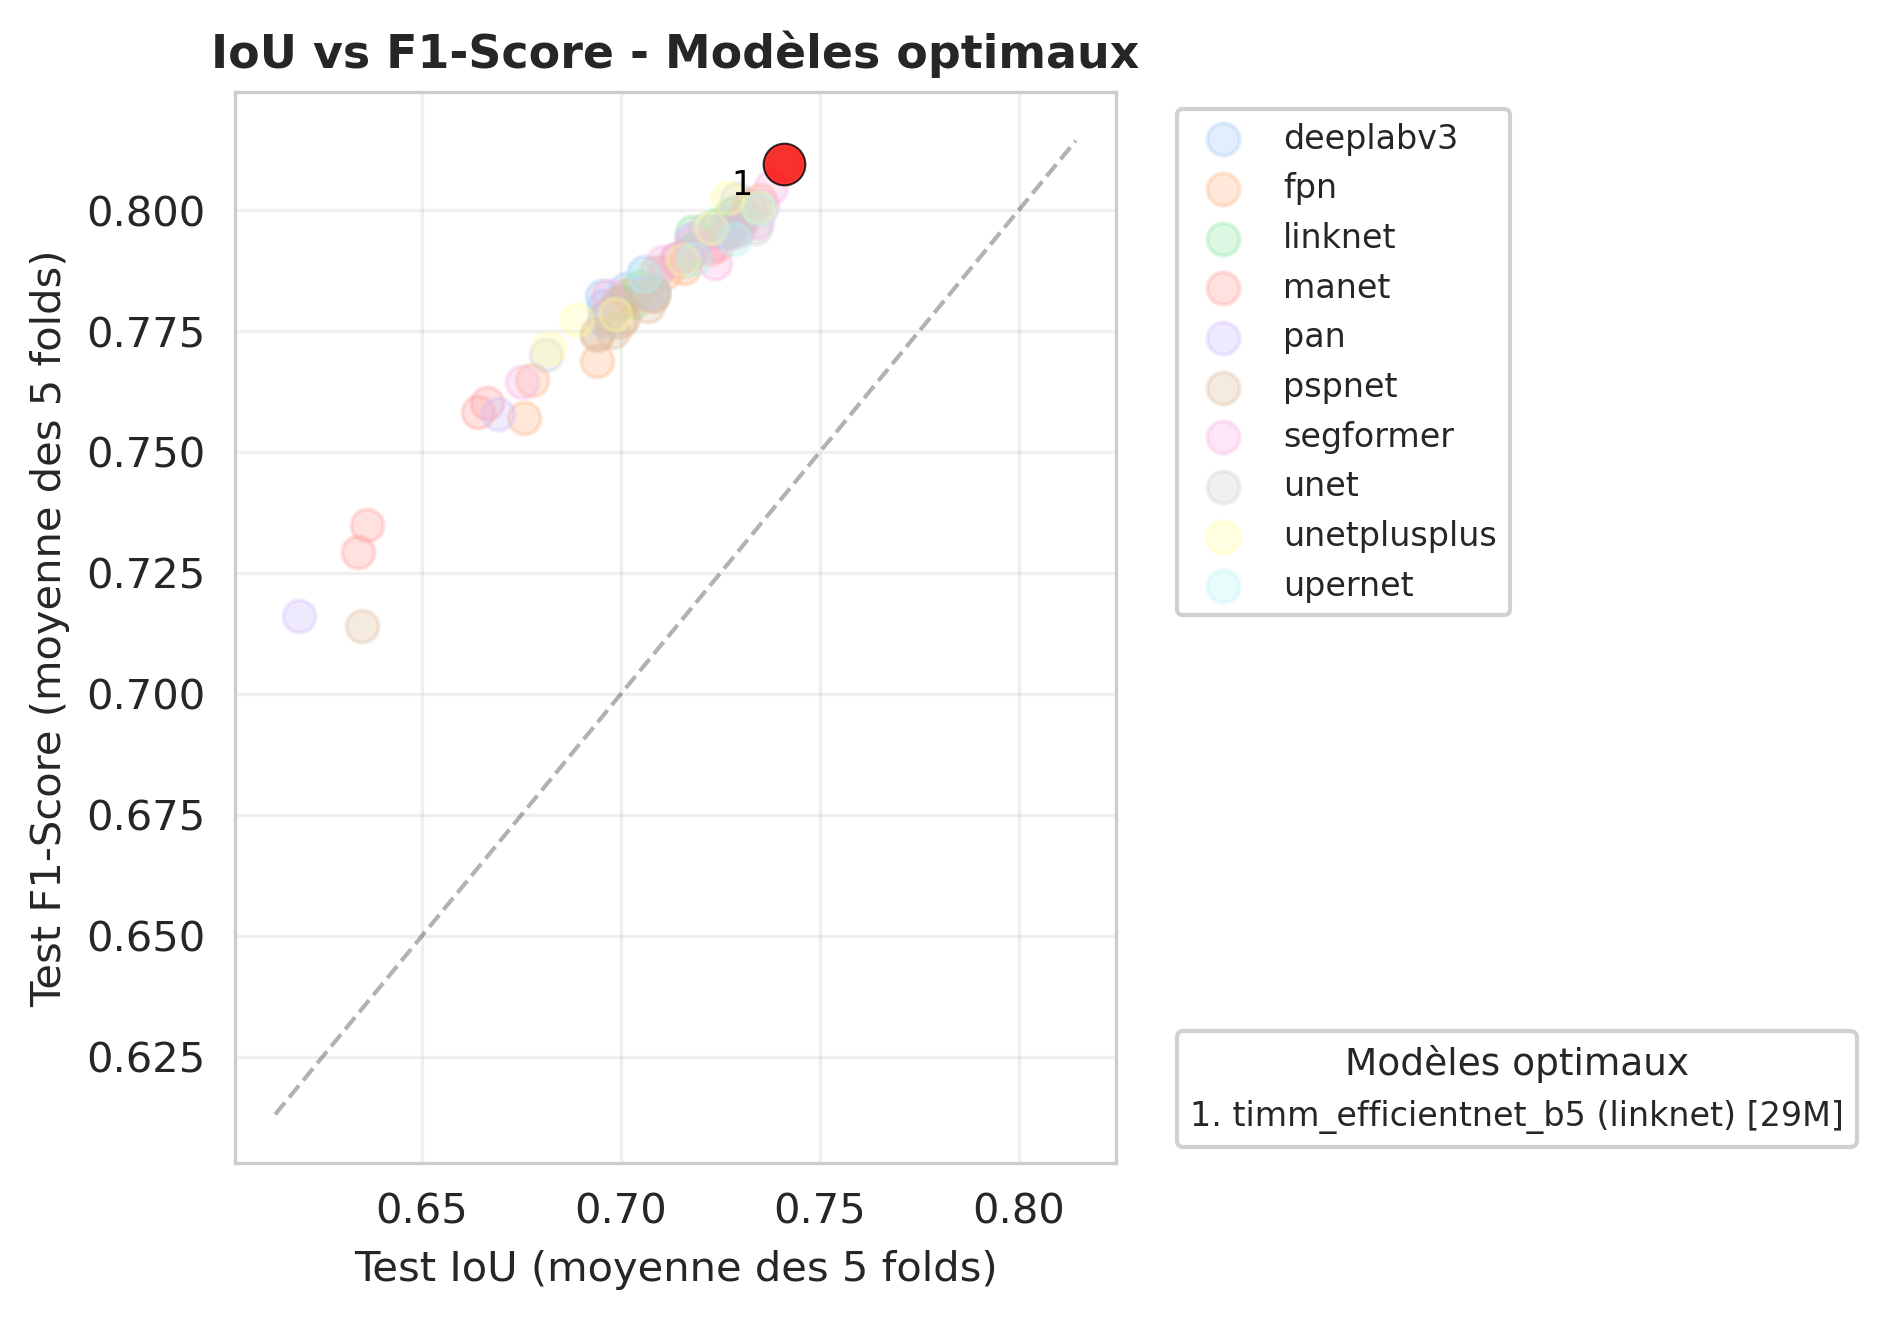
\includegraphics[width=0.8\textwidth]{ch4_10_01_iou_vs_eval_test_f1_score_mean.png}
    \caption{Relation entre IoU et F1-score. Les modèles YOLO (en orange) présentent un comportement distinct.}
    \label{fig:iou_vs_f1}
\end{figure}

\begin{itemize}
    \item \textbf{Modèles SMP} : Forte corrélation linéaire (R² > 0,95) entre IoU et F1-score
    \item \textbf{Modèles YOLO} : Décalage systématique avec F1-score inférieur pour un IoU donné
\end{itemize}

Cette divergence s'explique par la nature différente des architectures : YOLO optimise la détection d'instances tandis que SMP optimise directement la segmentation pixel par pixel.

\subsubsection{Analyse mAP multi-seuils}

Le Tableau~\ref{tab:map_analysis} présente l'évolution des performances selon différents seuils d'IoU :

\begin{table}[htbp]
    \centering
    \caption{Performances moyennes mAP à différents seuils}
    \begin{tabular}{lccccc}
        \toprule
        Architecture & mAP@50 & mAP@75 & mAP@95 & Chute relative \\
        \midrule
        UNet++ & 0,842 & 0,698 & 0,243 & -71\% \\
        DeepLabV3+ & 0,836 & 0,687 & 0,231 & -72\% \\
        YOLO & 0,798 & 0,612 & 0,187 & -77\% \\
        UNet & 0,821 & 0,654 & 0,208 & -75\% \\
        \bottomrule
    \end{tabular}
    \label{tab:map_analysis}
\end{table}

Les modèles SMP maintiennent mieux leurs performances aux seuils élevés, indiquant une segmentation plus précise des contours.

\subsection{Analyse par catégorie de taille}

L'analyse des performances par catégorie de taille (Figure~\ref{fig:models_by_size}) révèle des tendances intéressantes :

\begin{figure}[htbp]
    \centering
    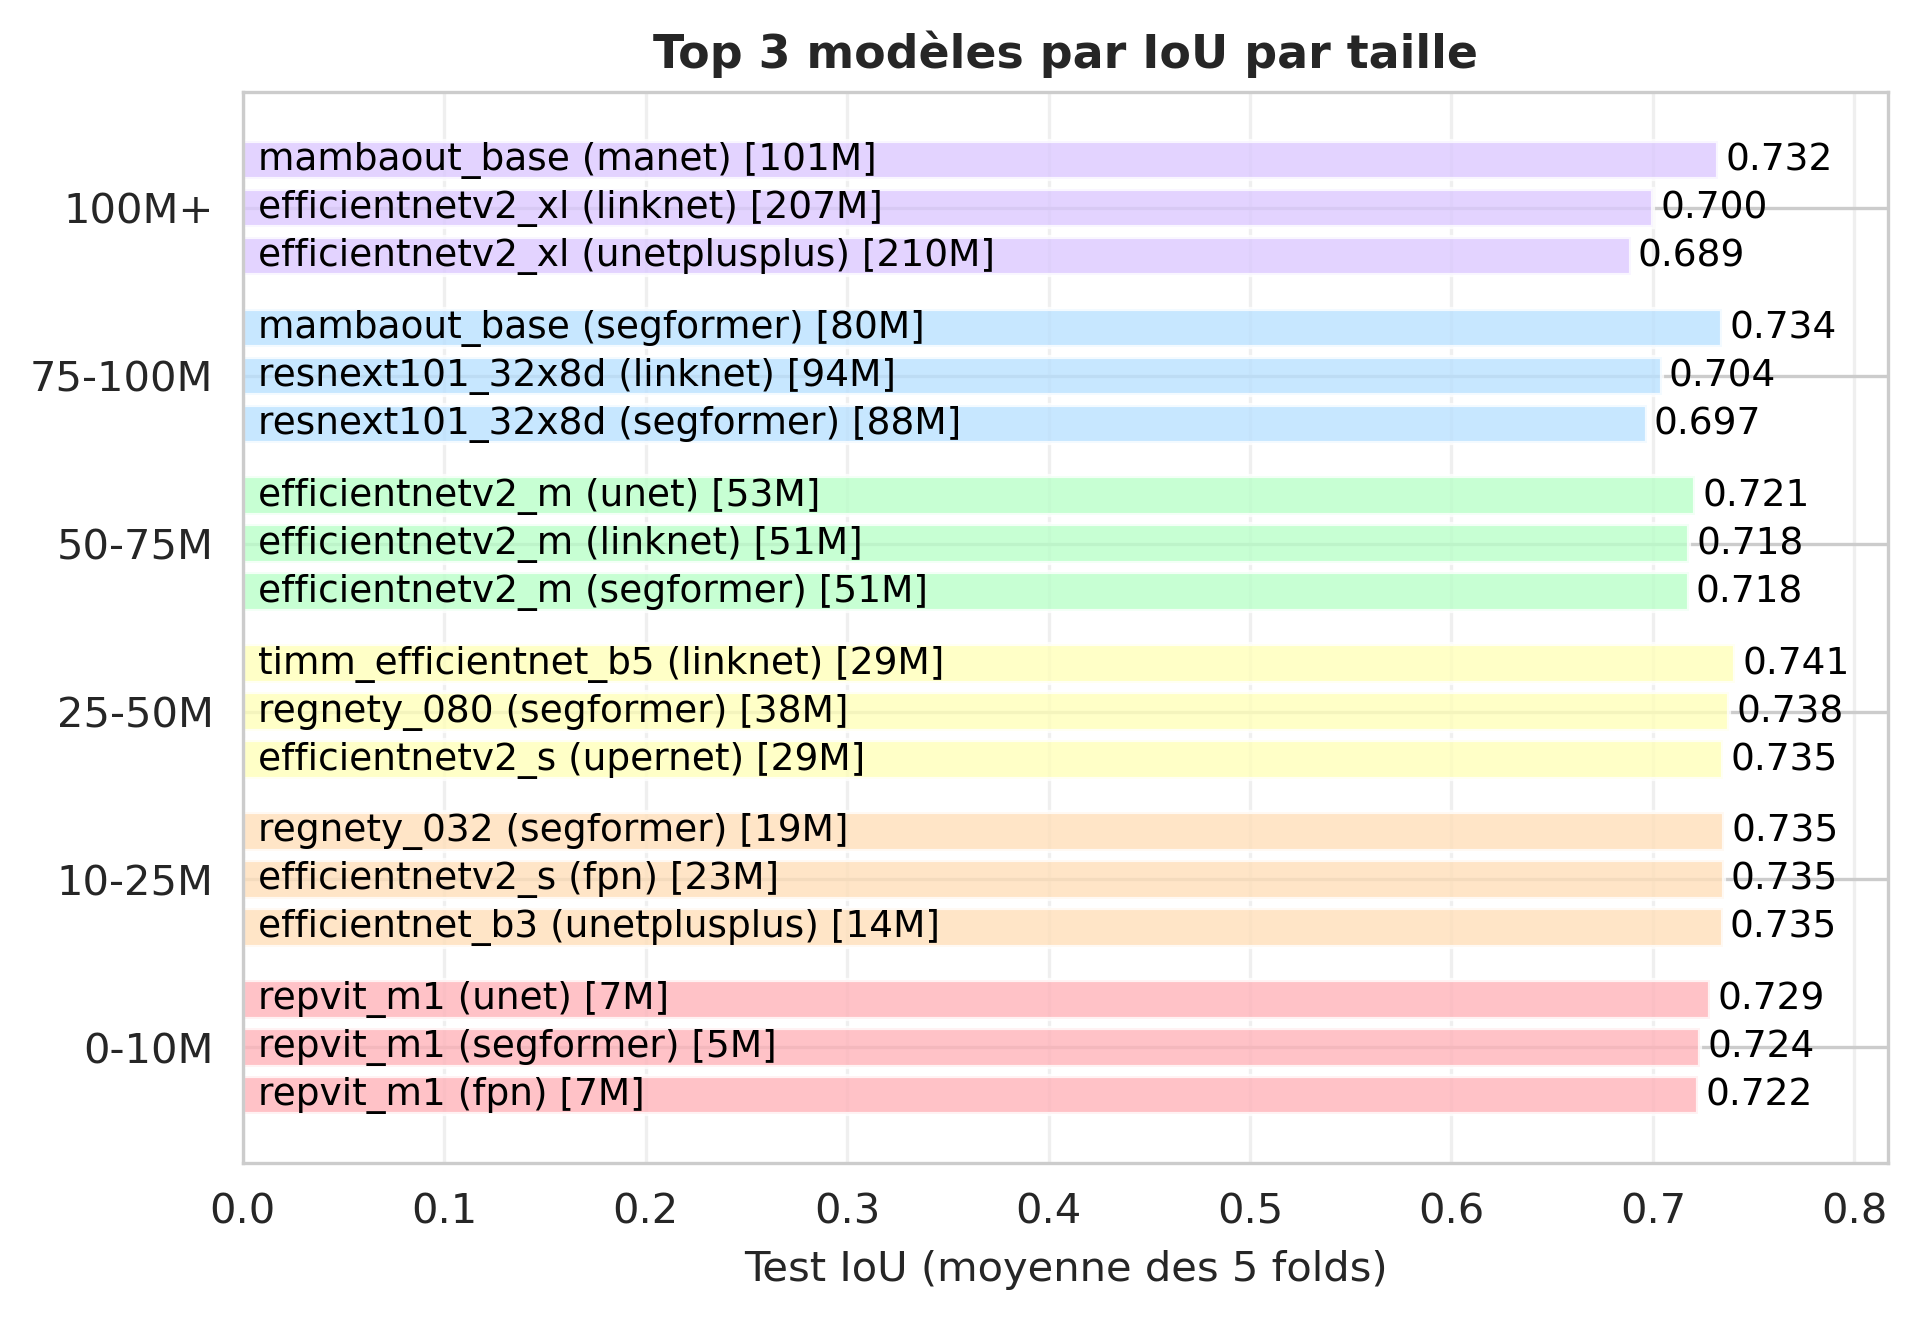
\includegraphics[width=\textwidth]{ch4_05_models_by_size_category_01_eval_test_iou_mean.png}
    \caption{Top 3 modèles par catégorie de taille (nombre de paramètres)}
    \label{fig:models_by_size}
\end{figure}

\begin{itemize}
    \item \textbf{0-10M params} : Dominée par YOLO12n et les combinaisons avec MobileNetV3
    \item \textbf{10-25M params} : Zone optimale avec les meilleures performances absolues
    \item \textbf{25-50M params} : Performances comparables mais temps d'entraînement supérieur
    \item \textbf{50M+ params} : Rendements décroissants évidents
\end{itemize}

\subsection{Recommandations par cas d'usage}

\subsubsection{Déploiement en production}

Selon les contraintes opérationnelles, différentes configurations sont recommandées :

\textbf{1. Performance maximale (serveur dédié)} :
\begin{itemize}
    \item \textbf{Modèle} : UNet++ + FastViT-T8
    \item \textbf{Caractéristiques} : IoU 0,742, 15,2M params
    \item \textbf{Justification} : Meilleures performances absolues avec taille raisonnable
\end{itemize}

\textbf{2. Temps réel (>30 FPS)} :
\begin{itemize}
    \item \textbf{Modèle} : YOLO12n ou YOLO12s
    \item \textbf{Caractéristiques} : IoU >0,70, <10M params
    \item \textbf{Justification} : Architecture optimisée pour l'inférence rapide
\end{itemize}

\textbf{3. Embarqué/Mobile} :
\begin{itemize}
    \item \textbf{Modèle} : UNet + MobileNetV3-large
    \item \textbf{Caractéristiques} : IoU 0,718, 7,0M params
    \item \textbf{Justification} : Conçu spécifiquement pour les contraintes mobiles
\end{itemize}

\textbf{4. Compromis optimal} :
\begin{itemize}
    \item \textbf{Modèle} : DeepLabV3+ + EfficientNetV2-S
    \item \textbf{Caractéristiques} : IoU 0,729, 22,5M params, 18,5h d'entraînement
    \item \textbf{Justification} : Équilibre idéal entre toutes les métriques
\end{itemize}

\subsubsection{Considérations pratiques}

Pour le déploiement à l'échelle du canton de Genève, plusieurs facteurs doivent être considérés :

\begin{enumerate}
    \item \textbf{Volume de données} : Avec environ 80 000 bâtiments, le temps d'inférence devient critique
    \item \textbf{Mise à jour} : Les modèles plus légers facilitent le ré-entraînement périodique
    \item \textbf{Interprétabilité} : Les architectures UNet offrent une meilleure visualisation des caractéristiques apprises
    \item \textbf{Robustesse} : La faible variance d'UNet++ suggère une meilleure généralisation
\end{enumerate}

\subsection{Synthèse et perspectives}

\subsubsection{Principaux enseignements}

Cette évaluation exhaustive permet de dégager plusieurs conclusions majeures :

\begin{enumerate}
    \item \textbf{Saturation des performances} : Au-delà de 25M paramètres, les gains deviennent négligeables
    \item \textbf{Importance de l'encodeur} : Les encodeurs récents (2021+) surpassent systématiquement les architectures classiques
    \item \textbf{Spécificité de la tâche} : Les architectures complexes (Transformers) n'apportent pas d'avantage décisif sur cette application
    \item \textbf{Trade-offs multiples} : Aucun modèle ne domine sur tous les critères simultanément
\end{enumerate}

\subsubsection{Limites et perspectives d'amélioration}

Plusieurs pistes pourraient améliorer les performances :

\begin{itemize}
    \item \textbf{Ensemble learning} : Combiner les prédictions des meilleurs modèles
    \item \textbf{Post-traitement} : Appliquer des filtres morphologiques pour raffiner les contours
    \item \textbf{Augmentation ciblée} : Enrichir le dataset avec des cas difficiles (ombres, reflets)
    \item \textbf{Multi-échelle} : Traiter les images à plusieurs résolutions
\end{itemize}

\subsection{Conclusion}

L'évaluation de 93 configurations sur le dataset de test révèle que les architectures modernes de segmentation atteignent des performances remarquables (IoU > 0,74) pour l'identification des espaces libres sur toitures. Le choix du modèle optimal dépend fortement des contraintes opérationnelles : UNet++ avec FastViT pour la performance pure, YOLO pour le temps réel, ou DeepLabV3+ avec EfficientNetV2 pour un compromis équilibré. Ces résultats valident la faisabilité d'un déploiement à grande échelle pour le cadastre solaire du canton de Genève.

\begin{itemize}
    \item \textbf{IoU (Intersection over Union)} : métrique principale mesurant le recouvrement entre les prédictions et les annotations de référence
    \item \textbf{mAP@k} : précision moyenne à différents seuils d'IoU (50\%, 55\%, ..., 95\%)
    \item \textbf{F1-score} : moyenne harmonique entre précision et rappel
    \item \textbf{Métriques classiques} : précision, rappel et exactitude
\end{itemize}

Les aspects computationnels ont également été mesurés :
\begin{itemize}
    \item Temps d'entraînement total pour les 5 plis
    \item Nombre de paramètres du modèle (en millions)
\end{itemize}









\subsection{Analyse qualitative}


% -----------------------------------------------------------------------------
\section{Application sur un quartier}
\subsection{Analyse qualitative}

% -----------------------------------------------------------------------------
\section{Analyse comparative des résultats}
\subsection{Généralisation du modèle}
\subsection{Limites identifiées}

% -----------------------------------------------------------------------------
\section{Synthèse}
\todo[inline]{Exemple de todo}